\documentclass[12pt,letterpaper]{article}

\newenvironment{proof}{\noindent{\bf Proof:}}{\qed\bigskip}

\newtheorem{theorem}{Theorem}
\newtheorem{corollary}{Corollary}
\newtheorem{lemma}{Lemma} 
\newtheorem{claim}{Claim}
\newtheorem{fact}{Fact}
\newtheorem{definition}{Definition}
\newtheorem{assumption}{Assumption}
\newtheorem{observation}{Observation}
\newtheorem{example}{Example}
\newcommand{\qed}{\rule{7pt}{7pt}}

\newcommand{\assignment}[4]{
\thispagestyle{plain} 
\newpage
\setcounter{page}{1}
\noindent
\begin{center}
\framebox{ \vbox{ \hbox to 6.28in
{\bf CS412: ntroduction to Data Mining \hfill #1}
\vspace{4mm}
\hbox to 6.28in
{\hspace{2.5in}\large\mbox{Problem Set #2}}
\vspace{4mm}
\hbox to 6.28in
{{\it Handed Out: #3 \hfill Due: #4}}
}}
\end{center}
}

\newcommand{\solution}[4]{
\thispagestyle{plain} 
\newpage
\setcounter{page}{1}
\noindent
\begin{center}
\framebox{ \vbox{ \hbox to 6.28in
{\bf CS412:   Introduction to Data Mining \hfill #4}
\vspace{4mm}
\hbox to 6.28in
{\hspace{2.5in}\large\mbox{#3}}
\vspace{4mm}
\hbox to 6.28in
{#1 \hfill {\it #2}}
}}
\end{center}
\markright{#1}
}

\newenvironment{algorithm}
{\begin{center}
\begin{tabular}{|l|}
\hline
\begin{minipage}{1in}
\begin{tabbing}
\quad\=\qquad\=\qquad\=\qquad\=\qquad\=\qquad\=\qquad\=\kill}
{\end{tabbing}
\end{minipage} \\
\hline
\end{tabular}
\end{center}}

\def\Comment#1{\textsf{\textsl{$\langle\!\langle$#1\/$\rangle\!\rangle$}}}


%\documentclass{article}
\usepackage{multirow}
\usepackage{amsmath}
\usepackage{amssymb}
\usepackage{algorithm}
\usepackage{algpseudocode}
\setlength{\parindent}{0pt}
\usepackage{graphicx}
\usepackage{ctable}
%\usepackage{fullpage}
%\usepackage{setspace} 
\usepackage{float}
%\usepackage{listings} 
%\usepackage{bbm}
\usepackage{bigstrut}
%\usepackage{caption}
%\usepackage{subcaption}
%\usepackage{algpseudocode}
%\usepackage{algorithm}
\usepackage{epstopdf}

\usepackage{listings}
\usepackage{color}
\usepackage[utf8]{inputenc}

\definecolor{dkgreen}{rgb}{0,0.6,0}
\definecolor{gray}{rgb}{0.5,0.5,0.5}
\definecolor{mauve}{rgb}{0.58,0,0.82}

\lstset{frame=tb,
  language=matlab,
  aboveskip=3mm,
  belowskip=3mm,
  showstringspaces=false,
  columns=flexible,
  basicstyle={\small\ttfamily},
  numbers=none,
  numberstyle=\tiny\color{gray},
  keywordstyle=\color{blue},
  commentstyle=\color{dkgreen},
  stringstyle=\color{mauve},
  breaklines=true,
  breakatwhitespace=true,
  tabsize=3
}


\oddsidemargin 0in
\evensidemargin 0in
\textwidth 6.5in
\topmargin -0.5in
\textheight 9.0in
\usepackage{multirow}
\usepackage{hyperref}

\hypersetup{colorlinks=true}
\usepackage{color}

\newenvironment{ans}{%
\vspace{5mm}
\textcolor{red}{{\sf Answer}}\\%
}
{%
}

\begin{document}


\solution{}{Due: 11/19/2015 11:59pm}{Assignment 4}{Fall 2015}
% Fill in the above, for example, as follows:
% \solution{Joe Smith}{\today}{1}{Fall 2012}

\pagestyle{myheadings}  % Leave this command alone

\paragraph*{General Instruction}
\begin{itemize}\vspace{-2mm}\setlength\itemsep{0mm}
	\item Errata: After the assignment is released, any further corrections of errors or clarifications will be posted at \href{https://piazza.com/class/idqujg4tiae3q0?cid=93}{the Errata page at Piazza}. Please watch it.
	\item Feel free to talk to other members of the class while doing the homework. We are more concerned that
	you learn how to solve the problem than that you solve it entirely on your own. You should, however, write the solution yourself. 
	\item Please use                            Piazza first if you have questions about the homework. Also feel free to send us e-mails and come to office hours. 
	\item For each question, you should show the necessary calculation steps and reasoning---not only final results. Keep the solution brief and clear.
	\item For a good balance of cognitive activities, we label each question with an activity type:
	\begin{itemize}
		\item {\bf L1 (Knowledge)} Definitions, propositions, basic concepts.
		\item {\bf L2 (Practice)} Repeating and practicing algorithms/procedures.
		\item {\bf L3 (Application)} Critical thinking to apply, analyze, and assess.
	\end{itemize}
\end{itemize}
\paragraph*{Assignment Submission}
\begin{itemize}\vspace{-2mm}\setlength\itemsep{0mm}
	\setlength{\itemsep}{2pt}
	\item Please submit your work before the due time. \textbf{We do NOT accept late submission!}
	\item 
	Please submit your answers electronically via  \href{http://compass2g.illinois.edu}{Compass}. Contact CITES/TAs if you have technical difficulties in submitting the assignment.
	\item For this assignment, {\bf typeset} your answers and submit it in a {\bf single PDF file}. \textbf{Handwritten answers or hand-drawn pictures} \textbf{are not acceptable}.
\end{itemize}

\section{Constraint pattern mining (10 points)}
For the following constraints, write down your answer if they are (strongly convertible, convertible) Anti-monotone, Monotone or Succinct. 
\textbf{Purpose} 
\begin{itemize}\vspace{-2mm}\setlength\itemsep{-1mm}
\item Have a better understanding of constraint pattern mining.
\end{itemize}
\textbf{Requirements}
\begin{itemize}\vspace{-2mm}\setlength\itemsep{-1mm}
\item A short explanation to justify if the constraint belongs to \textbf{EACH} type is required. To show a constraint is not of one type, a simple example is enough.
\end{itemize}

\begin{itemize}
\item[a.] (2', L1) for a set of values $S$, and a value $v$, constraint $v \in S$
\item[b.] (2', L1) for a set of values $S$, and a value $v$, constraint $max(S) \geq v$
\item[c.] (2', L1) for a set of values $S$, and a value $v$, constraint $max(S) \leq v$
\item[d.] (4', L1) for a set of values $S$, and a value $v$, constraints $avg(S) \geq v$ and $avg(S) \leq v$
\end{itemize}



\section{Advanced pattern mining (10 points)}
For each question below, indicate if the statement is \textbf{true} or \textbf{false}.\\
\textbf{Purpose} 
\begin{itemize}\vspace{-2mm}\setlength\itemsep{-1mm}
\item Have a better understanding of advanced pattern mining.
\end{itemize}
\textbf{Requirements}
\begin{itemize}\vspace{-2mm}\setlength\itemsep{-1mm}
\item For each sub-question, select \textbf{true (T)} or \textbf{false (F)} and also write down a brief explanation. You will \textbf{NOT} get credit without an explanation. 
\end{itemize}
\begin{itemize}
    \item[a.] (2', L2) \textbf{T/F.}  Convertible constraints cannot be exploited in an Apriori mining algorithm.
    \item[b.] (2', L2) \textbf{T/F.}  In \textit{PrefixSpan}, physical project is not used because of its slow performance.
    \item[c.] (2', L1) \textbf{T/F.}  Mining closed frequent graphs only is lossless compression of the graph database.
    \item[d.] (2', L3) \textbf{T/F.}  In sequential pattern mining, the number of length-2 candidates generated from $x$ frequent length-1 sequences is $\frac{3}{2}x^2 - \frac{1}{2}x$
    \item[e.] (2', L3) \textbf{T/F.}  For nontrivial constraints (not every possible pattern satisfies the constraint), it cannot be monotone and anti-monotone at the same time.
\end{itemize}



\section{Sequential pattern mining (30 points)}
Use a toy dataset to perform sequential pattern mining algorithms.
\textbf{Purpose} 
\begin{itemize}\vspace{-2mm}\setlength\itemsep{-1mm}
\item Work on sequential pattern mining using \textit{GSP} and \textit{PrefixSpan}
\end{itemize}
\textbf{Requirements}
\begin{itemize}\vspace{-2mm}\setlength\itemsep{-1mm}
\item Write down each step as detail as possible.
\end{itemize}

Suppose a toy sequence database $D$ contains three sequences as follows. Let the minimum support be 3.

 \begin{tabular}{c|l}
 % after \\: \hline or \cline{col1-col2} \cline{col3-col4} ...
 customer\_id & shopping sequence \\\hline
  1 & $(bc) (de) f$ \\
  2 & $ bc d ef$ \\
  3 & $(bc) d b e g f$ \\\hline
 \end{tabular}\\

The following questions require you to perform GSP algorithm.

\begin{enumerate}
\item [(1)] (5', L2) Scan database once, list length-1 sequential pattern candidates $C_1$ and the result $L_1$ after pruning. 
\item [(2)] (5', L2) Followingly, generate $C_2$, and $L_2$. \textit{Hint: do not miss any candidates in $C_2$}
\item [(3)] (5', L2) Now, generate $C_3$, $L_3$, $C_4$, $L_4$ and longer candidates/results until the algorithm terminates.
\end{enumerate}


\section{Decision Trees (20 points)}
ID3 is a simple algorithm for decision tree construction using information gain. The steps of the ID3 algorithm are similar to those introduced in the lecture and described below for your reference. Your task is to use ID3 to build a decision tree that predicts whether a candidate will be accepted to the PhD program of University X, given the student's information including her GPA, university, any publications, and recommedation letter. The training and testing data are given in Table~\ref{tab:dt} and Table~\ref{tab:dt-test}.\\

\textbf{Purpose} 
\begin{itemize}
    \item Understand and practice basic decision tree construction, calculation of information gain measures, and classifier evaluation.
\end{itemize}

\textbf{Requirements}
\begin{itemize}
    \item Show the calculations for selecting the decision tree attributes and the labels for each leaf.
\end{itemize}

\begin{table}[!h]
    \centering
    \label{tab:dt}
    \begin{tabular}{l|cccc|c}
        \hline
        
        \hline
        {\bf id} & {\bf GPA} & {\bf univ}  & {\bf published} & {\bf recommendation} & {\bf accepted} \\ \hline
        1 & 4.0 &  top-10 &  yes &  good & yes  \\ 
        2& 4.0&  top-10&  no&  good& yes  \\ 
        3& 4.0&  top-20&  no&  normal&  yes  \\ 
        4& 3.7&  top-10&  yes&  good&  yes  \\ 
        5& 3.7&  top-20&  no&  good&  yes  \\ 
        6& 3.7&  top-30&  yes&  good&  yes  \\ 
        7& 3.7&  top-30&  no&  good& no   \\ 
        8& 3.7&  top-10&  no&  good& no   \\ 
        9& 3.5&  top-20&  yes&  normal& no   \\ 
        10& 3.5&  top-10&  no&  normal& no   \\ 
        11& 3.5&  top-30&  yes&  normal& no  \\ 
        12& 3.5&  top-30&  no&  good& no  \\ 
        \hline
        
        \hline
    \end{tabular}
    \caption{Training Data for the decision tree problem}
\end{table}

\begin{table}[!h]
    \centering
    \label{tab:dt-test}
    \begin{tabular}{l|cccc|c}
        \hline
        
        \hline
        {\bf id} & {\bf GPA} & {\bf univ}  & {\bf published} & {\bf recommendation} & {\bf accepted} \\ \hline
        1& 4.0 &  top-10 &  yes &  good & yes  \\ 
        2& 3.7&  top-30&  yes&  good&  yes  \\
        3& 3.5&  top-30&  yes&  good&  yes  \\      
        4& 3.7&  top-10&  no&  good& no   \\ 
        5& 3.5&  top-30&  no&  good& no  \\ 
        \hline
        
        \hline
    \end{tabular}
    \caption{Testing Data for the decision tree problem}
\end{table}

\begin{algorithm}[!h]
    \begin{algorithmic}
    \Function{ID3}{$tuples$, $TargetAttrib$, $PredictAttribs$}
        \State Create root $r$ of the tree;
        \If{all $tuples$ are positive}
            \State \Return $r$ with label `+';
        \EndIf
        \If{all $tuples$ are negative}
            \State \Return $r$ with label `-';
        \EndIf
        \If{$PredictAttribs$ are empty}
            \State \Return $r$ with label as most common among $tuples$;
        \EndIf

        \State $A\leftarrow$ the attribute in $PredictAttribs$ that best classifies the samples in terms of information gain;
        \State Let $A$ be the decision attribute of root node $r$;
        \For{each possible value $v_i$ of $A$}
            \State Add a new branch below $r$ corresponding to $A=v_i$;
            \State Let $tuples(v_i)$ be the subset of $tuples$ with value $v_i$ for $A$;
            \If{$tuples(v_i)$ is empty}
                \State Add a leaf node below this new branch, with label as the most common label in $tuples$;
            \Else
                \State Add the subtree ID3($tuples(v_i)$, $TargetAttrib$, $PredictAttribs – \{A\}$) below this new branch;
            \EndIf
        \EndFor
        \State \Return the tree rooted at $r$;
    \EndFunction
  \end{algorithmic}
\end{algorithm}





\begin{itemize}
    \item[a.] (5', L2) Using ID3 to construct a decision tree using the training data in Table~\ref{tab:dt}. When multiple attributes has best information gain, choose the one whose name appears earliest in alphabetical order. When there is a tie for the majority labels, choose `-'. Show the final decision tree, and the calculations to derive that tree.
    
    \item[b.] (5', L2)Evaluate your constructed decision tree using the testing data in Table~\ref{tab:dt-test} using precision and recall. Show your steps and calculations.
    \item[c.] (5', L2) What is the time complexity of training a decision tree using ID3 on a dataset with $n$ data records and $m$ attributes each having $p$ possible values? Show your analysis.
    \item[d.] (5', L3) Each root-to-leaf path in any decision tree can be converted into a rule, such as a path $A_1\xrightarrow{=True}A_2\xrightarrow{=False} class=+1$ can be converted to the rule ``If attribute $A_i$ is true and attribute $A_2$ is false, then the instance has class $+1$''. Please do/answer the following:
        \begin{itemize}
            \item[1.] Generate the rules for each leaf of your constructed decision tree.
            \item[2.] Is it possible to construct a decision tree from a set of rules? Explain your answer.
        \end{itemize} 
% \item[c.] What classification rules can you derive from your constructed decision tree by following the?
\end{itemize}


\section{AdaBoost (15 points)}
You will be guided through the steps of building an ensemble classifier using AdaBoost. The data points to be classified are given in Table~\ref{tab:ab}. Each classifier in the ensemble will have the following form: if $x>a$, label $1$; else $-1$, where $a$ is a constant for you to figure out. That is, the hypothesis of the classifier is a line parallel to the $y$-axis. Assume that data weight distribution $D_1$ at the initial round of AdaBoost is uniform.\\

\begin{table}[!h]
    \label{tab:ab}
    \centering
    \begin{tabular}{l|cc|c}
    \hline

    \hline
    \textbf{id} & $x$ & $y$ & {\bf label}\\
    \hline
         1 & 1.0 & 0.5 & +1\\
         2 & 2.2 & 1.0 & +1\\
         3 & 2.7 & 2.0 & +1\\
         4 & 0.5 & 1.5 & -1\\
         5 & 1.2 & 2.3 & -1\\
         6 & 1.5 & 2.7 & -1\\
    \hline

    \hline
    \end{tabular}
    \caption{Data points for the AdaBoost problem}    
\end{table}

\textbf{Purpose} 
\begin{itemize}
\item Understand and practice AdaBoost algorithm by walking through the steps.
\end{itemize}

\textbf{Requirements}
\begin{itemize}
\item Show all the steps and calculations needed to derive each classifier.
\end{itemize}

\begin{itemize}
    \item[a.] (3', L3) Find a classifier $h_1$ that has minimum weighted error for the given data and the weight distribution $D_1$. Show your steps method to get $h_1$.
    \item[b.] (2', L2) What is the weighted error rate of classifier $h_1$ with data weights $D_1$?
    \item[c.] (2', L2) After re-weighting of the data with $h_1$, what's the new data weight distribution $D_2$ for round 2? Normalize the weights so that they sum to 1.
    \item[d.] (3', L3) Like in (a), find a classifier $h_2$ that has the minimum weighted error rate for the data weight distribution $D_2$.
    \item[e.] (4', L2) What is accuracy of the ensemble classifier that combines $h_1$ and $h_2$ on the given data?
\end{itemize}

\section{Bayes Classifier (15 points)}
Give records about whether two people played tennis ({\tt play\_tennis}, the target attribute) under certain weather in terms of  attributes ({\tt outlook, temperature, wind}), you will train a Naive Bayes classifier to predict whether they will play tennis given a weather. The training data are given in Table~ref{tab:bayes}.\\

\begin{table}[!h]
    \label{tab:bayes}
    \centering
    \begin{tabular}{l|ccc|c}
    \hline

    \hline
    % Day    Outlook    Temperature      Humidity    Wind       PlayTennis
    \textbf{id} & \textbf{outlook} & \textbf{temperature} & \textbf{wind} & \textbf{play tennis}\\
    \hline
        1 & sunny & hot & weak & no\\
        2 & sunny & hot & strong & no\\
        3 & overcast & hot & weak & yes\\
        4 & rain & mild & weak & yes\\
        5 & rain & cool & weak & yes\\
        6 & rain & cool & strong & no\\
        7 & overcast & cool & strong & yes\\
        8 & sunny & mild & weak & no\\
        9 & sunny & cool & weak & yes\\
        10 & rain & mild & weak & yes\\
        11 & sunny &mild & strong & yes\\
        12 & overcast & mild & strong &  yes\\
        13 & overcast & hot & weak & yes\\
        14 & rain & mild & strong & no\\
    \hline

    \hline
    \end{tabular}
    \caption{Training data for the Bayes classfier problem}
\end{table}

\textbf{Purpose} 
\begin{itemize}
\item Understand and practice the principles of Naive Bayes classifier and its training algorithm.
\end{itemize}

\textbf{Requirements}
\begin{itemize}
\setlength{\itemsep}{1pt}
\item Show the steps and calculations to derive the classifier.
\item Follow the {\it given} steps to calculate the probabilities for making predictions.
\item Show the formulas you used to calculate the results.
\end{itemize}

%TODO: laplacian correction
\begin{itemize}
    \item[a.]  (3', L2) What is the prior probability of {\tt play\_tennis} being {\tt yes}/{\tt no} estimated from the data?
    \item[b.] (3', L2) What is the conditional probability of attribute in {\tt outlook} taking each of the values ({\tt sunny, rain, overcast}), given {\tt play\_tennis= yes}? Also calculate conditional probabilities for attributes ({\tt temperature, wind}) taking their possible values given {\tt play\_tennis=yes}.
    \item[c.] (3', L2) Calculate the conditional probabilities in (b) by replacing the condition by {\tt play\_tennis= no}.
    \item[d.] (3', L2) Based the results you got from (a)-(c), given attribute values ({\tt outlook= sunny, temperature= cool, wind= strong}), calculate the probability of {\tt play\_tennis= yes}. What will the probability become if {\tt outlook=rain, temperature=cool, wind=weak}?
    \item[e.] (3', L2)Given $n$ training data records each having $m$ attributes:
    \begin{itemize}
        \item[1.] What is the time complexity of training a Naive Bayes classifier? Show your analysis.
        \item[2.] How will the complexity be affected without assuming the attributes are conditionally independent given the label? 
    \end{itemize}  
    % \item[e.] Use an alternative method to calculate the probabilities asked in (d) {\it without} using the conditional probabilities calculated in (c).
\end{itemize}



\section{Mini Machine Problem (10 points)}
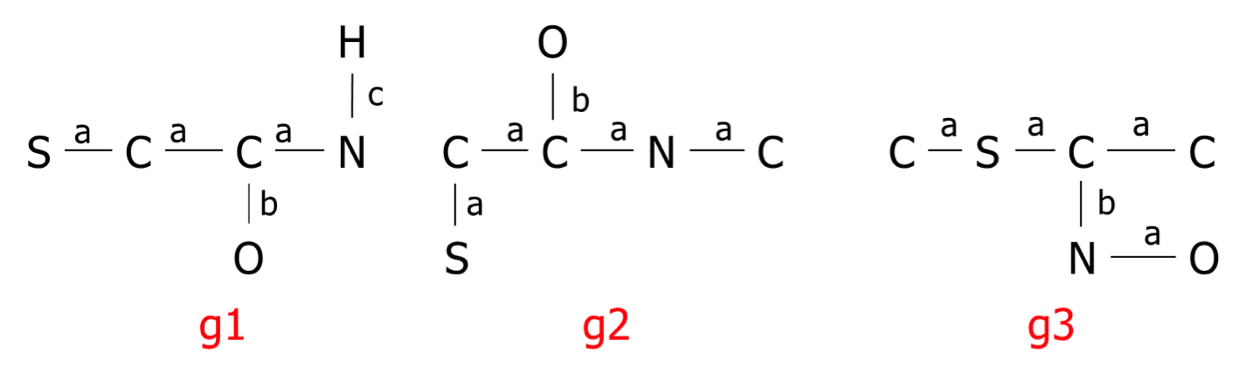
\includegraphics[scale=0.5]{gspan.png} 

gSpan is an algorithm for mining frequent graph patterns. On the course page, download the gSpan package and complete the following questions.

\textbf{Purpose} 
\begin{itemize}\vspace{-2mm}\setlength\itemsep{-1mm}
\item Work on graph mining using \textit{gSpan}
\item Know how to convert graph and pattern into files of correct format
\end{itemize}

\textbf{Requirements}
\begin{itemize}\vspace{-2mm}\setlength\itemsep{-1mm}
\item For each question, draw all the pattern graphs as given from the gSpan algorithm.
\end{itemize}

Here is three molecular formulas. Using gSpan to find \textbf{ALL} patterns that:
\begin{itemize}
\item[(1)] appear at least in two molecular structures.
\item[(2)] appear in all three molecular structures.
\end{itemize}

Note that the executable binary we have is compiled on Linux. You will need to use a Linux machine (such as EWS) to run the algorithm (though you can hack a little bit to run Linux binary on Mac by emulating --- do a Google search for related pages)
    

\end{document}